Calcule el volumen generado por una elipse horizontal con semieje mayor $a$ y semieje menor $b$ al rotar alrededor del eje $x$.

\nopagebreak
\begin{align*}
\text{Elipse: } \frac{x^2}{a^2} + \frac{y^2}{b^2} = 1 \implies y^2 = b^2(1 - x^2/a^2). \\
V &= \pi \int_{-a}^{a} y^2 \, dx \\
&= \pi \int_{-a}^{a} b^2 \left(1 - \frac{x^2}{a^2}\right) \, dx \\
&= 2\pi b^2 \int_{0}^{a} \left(1 - \frac{x^2}{a^2}\right) \, dx \\
&= 2\pi b^2 \left[ x - \frac{x^3}{3a^2} \right]_{0}^{a} \\
&= 2\pi b^2 \left( a - \frac{a}{3} \right) = 2\pi b^2 \left(\frac{2a}{3}\right) = \frac{4}{3}\pi ab^2
\end{align*}

\[
\boxed{\displaystyle \frac{4}{3}\pi ab^2}
\]

\begin{center}
    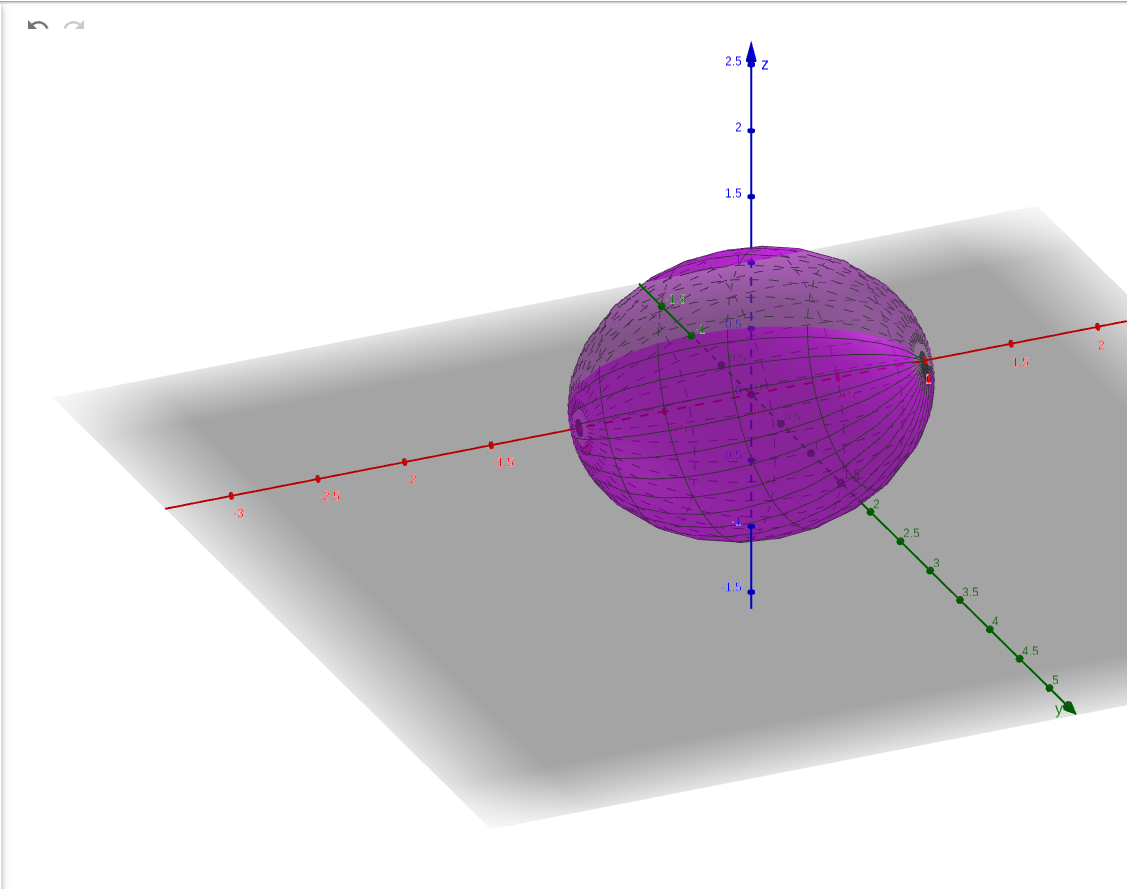
\includegraphics[width=0.5\textwidth]{Graficas/ejer32.png}
\end{center}
